\section{Implementation}\label{sec:implementation}
For the replication of the results presented in section~\ref{sec:reading-and-theory} I decided to use pytorch\footnote[1]{\href{https://pytorch.org/}{https://pytorch.org/}} due to personal preference and previous experience.
The implementation consists of a library which can be found in the \codeword{src} folder.
The library contains the implementation of all models, datasets, training and evaluation methods.
Further, a notebook is provided in the root directory, offering access to the implemented library functions and using them for training, evaluation and visualisation.
In the following firstly the two implemented datasets CIFAR-10 and FashionMNIST are introduced in section~\ref{subsec:datasets}, then the implemented models and their respective architecture is presented in section~\ref{subsec:models}.
Section \ref{subsec:training} describes the training process.
Finally, the results achieved by the models are discussed in section~\ref{subsec:evaluation}.

\subsection{Datasets}\label{subsec:datasets}
The following introduces the CIFAR-10 and FashionMNIST dataset.

\subsubsection{CIFAR-10}
The CIFAR-10~\cite{CIFAR10} is a dataset for the task of classification consisting of a total of 60.000 images from 10 different classes including various vehicles and animals.
The individual images have a size of $32\times 32$ and are given as RGB images.
The training split contains 50.000 images and the test split the remaining 10.000.
As my exploration of the hyperparameter space is extremely limited I decided against using an additional validation split as it is highly unlikely for the hyperparameters to overfit.

\subsection{FashionMNIST}
The FashionMNIST~\cite{DBLP:journals/corr/abs-1708-07747} dataset is a dataset for the task of classification dataset inspired by the original MNIST dataset which contains handwritten digits.
The dataset consists of 10 classes each representing a fashion item.
FashionMNIST contains a total of 60.000 training images and an additional 10.000 test images.
Again, I decided not to use a validation split.
The images are given as $28\times 28$ gray-scale images.
Figure~\ref{fig:datasets_ex} shows three examples from both of the datasets.
\begin{figure}[t]
    \centering
    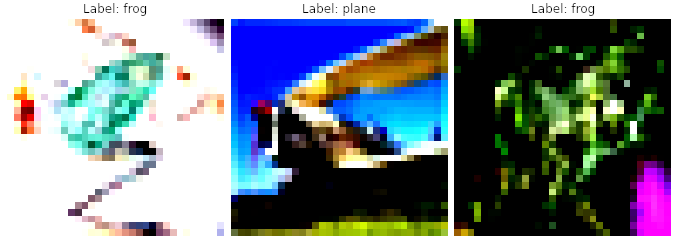
\includegraphics[width=.45\textwidth]{res/CIFAR.png}
    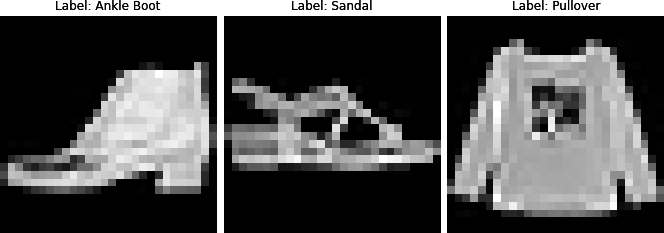
\includegraphics[width=.45\textwidth]{res/MNIST.png}
    \caption{Three examples from the CIFAR-10 dataset with their respective labels on the left and the MNIST dataset on the right.}
    \label{fig:datasets_ex}
\end{figure}

\subsection{Models}\label{subsec:models}
The models implemented in \codeword{src/models} contain a ResNet-34~\cite{he2015deep}, a implementation of the GroupNorm layer and two simple CNNs SimpleNet and SimpleNetv2.
My implementation of the GroupNorm utilizes the code provided in the original paper~\cite{DBLP:journals/corr/abs-1803-08494} and wrapped it inside a module for the convenient management of parameters.
For the ResNet the basic residual block proposed in~\cite{he2015deep} and the ResNet-34 architecture is used.
I tried using a ResNet as it is a well established architecture achieving good results on many tasks, however I was unable to train the smaller batch sizes using ResNet as the time required for training was not feasible for me.
However, I decided to use the results of the ResNet-34 as baseline to compare to other models.\\
The SimpleNetv2 consists of three SimpleBlocks, their architecture is shown in figure~\ref{fig:simplenet} on the left.
The SimpleBlock contains two stacked convolutions.
After the first convolution, the number of input channels is doubled.
After each convolution a normalization layer and ReLU are applied.
Finally, each SimpleBlock is terminated by a Max-Pooling operation, reducing the spatial resolution by a factor of two.
The full architecture of the SimpleNetv2 is shown in figure~\ref{fig:simplenet} on the right.
The first basic block increases the number of channels from 3 to 32.
The three basic blocks achieve an output stride of 8.
Finally, two linear layers using ReLU and no activation respectively, with the first one having 1024 neurons and the output having 10 neurons.
\begin{figure}[h]
    \centering
    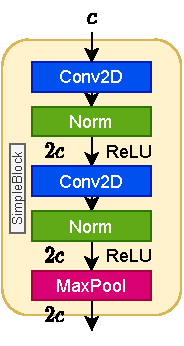
\includegraphics[width=.3\textwidth]{res/basicBlock.pdf}
    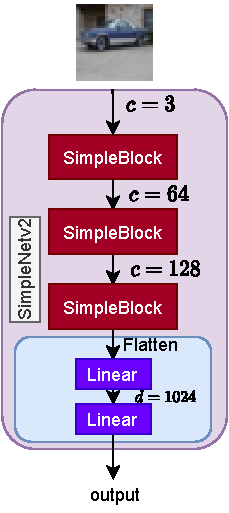
\includegraphics[width=.25\textwidth]{res/SimpleNetv2.pdf}
    \caption{Architecture of the simple basic block on the left and the SimpleNetv2 on the right.}
    \label{fig:simplenet}
\end{figure}

\subsection{Training}\label{subsec:training}
The training procedure described in the following is used for both the CIFAR-10 model and the FashionMNIST model.
However, the evaluation solely considers the CIFAR-10 dataset.
The training was conducted on a Nvidia GTX 1660ti with 6GB of VRAM.
As a loss function a standard cross-entropy loss is utilized.
For optimization an Adam optimizer with weight decay was employed with the following parameters $\text{lr}=0.001, \beta_1=0.9, \beta_2=0.999, \varepsilon=1\cdot 10^{-8}$ and for the weight decay $\lambda=0.01$.
I experimented with different optimizers including Adam without weight decay and SGD but the above named configuration was the most stable and achieved the best results.
Furthermore, a cosine annealing learning rate scheduler is used.
The SimpleNetv2 network was trained for a total of 30 epochs, whereas the ResNet-34 was trained for a total of 200 epochs on the dataset.
During training the following batch sizes are used $\{2, 4, 8, 16, 32, 64\}$.
The models employing group normalization are trained using a group size of 16.

\subsection{Evaluation}\label{subsec:evaluation}
After training a total of thirteen networks on the CIFAR-10 dataset using the training procedure described above the following results are obtained.
\begin{figure}[h]
    \centering
    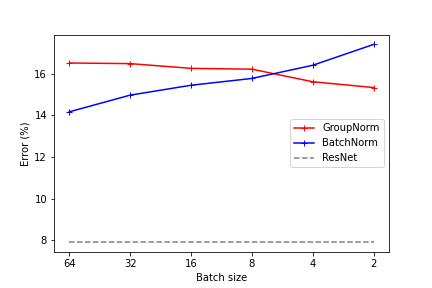
\includegraphics[width=.85\textwidth]{res/plot.png}
    \caption{Evaluation}
    \label{fig:eval}
\end{figure}
Figure~\ref{fig:eval} displays the achieved results.
The x-Axis marks the different batch sizes, the y-Axis the error of the model on the test split.
The result of the best ResNet-34 is shown as the dashed gray line and is used as a baseline.
The batch norm and the group norm are shown in blue and red respectively.
The figure clearly shows that the model using batch norm drastically improves when the batch size increases.
Further, the group norm degrades with a higher batch size but not nearly as bad as the batch norm.
However, this behaviour is not intuitive as the batch size should not directly affect the group normalization.
For small batch sizes (e.g. 2 and 4) the group norm models are able to outperform the batch norm models.
For larger batches sizes (batch size $> 4$) the batch norm model starts to outperform the group norm.
Compared to the results obtained in the original paper the difference between batch and group norm for small batch sizes is significantly smaller.
My explanation for this behaviour is that this is due to the dataset.
Compared to ImageNet, CIFAR-10 is a significantly easier dataset on which a less complex model is still able to achieve a good performance.
This idea is supported by the fact that the difference between batch and group norm on the FasionMNIST dataset is even smaller.
During my evaluation of the FashionMNIST dataset all models were within $1.5\%$ but the order was still as expected, meaning for batch size 2 the group norm outperformed the batch norm.
Furthermore, during my experiments with the ResNet-34 on CIFAR-10 the difference between group and batch norm appeared to be similar to the results achieved by the SimpleNetv2.
However, I do not have an explanation for the deterioration of the group norm for larger batch sizes.
